\documentclass[a4paper,prd,twocolumn,nofootinbib,superscriptaddress,floatfix]{revtex4}
%\documentclass[prd,twocolumn,nofootinbib,showpacs]{revtex4-1}

\usepackage{cancel}
\usepackage{graphicx}
\usepackage{epsfig}
\usepackage{amsmath,amsfonts,amssymb}
\usepackage[latin9]{inputenc}
\usepackage[portuguese]{babel} 
\usepackage{algorithm}
\usepackage{algorithmic}


\hyphenation{}
\begin{document}

%\linenumbers

\title{Lowest Common Subsequence - Serial and Parallel Implementation}

\author{Jos� Antunes} 
\author{C�sar Alves}
\author{Mauro Machado}

\affiliation{Departamento de F�sica, Instituto Superior T�cnico, Universidade de Lisboa, Lisboa, Portugal}

\begin{abstract}
The Longest Common Subsequence (LCS) was implemented in a serial and parallel fashion. Our serial implementation creates a matrix that is run line by line. In the parallel version each anti-diagonal was calculated in sequence with each value being calculated in parallel.
\end{abstract}

\maketitle

\section{Introduction}
With this work we wish to study the difference in execution time between the serial and parallel implementation of the Longest Common Subsequence (LCS) algorithm. This is a relevant algorithm in the bioinformatics field where a comparison between two DNA sequences is needed.

Problems appear when sequences become very large and the serial implementation of the code starts to have a very long execution time.

Processors have evolved more in the direction of having multiple cores over faster speeds and, as such, the trivial answer to these longer execution times is to have a parallel approach to the problem.

The LCS algorithm takes two sequences, $X$ and $Y$, of different lengths and will use a matrix to compare them. The matrix will be filled with integer values depending on how each element and the previous ones compare to each other.

The basic structure of the algorithm is the following:

\[ c(i, j) = \left\{ 
  \begin{array}{l l}
    0 & \text{if $i, j = 0$}\\
    c(i-1, j-1) + 1 &  \text{if $i, j > 0$ $x_i = y_j$}\\
    max( c(i-1, j); c(i, j-1) ) &  \text{if $i, j > 0$ $x_i \neq y_j$}
  \end{array} \right.\]
and this creates a matrix which will give the longest subsequence.

\begin{figure}[h!]
  \centering
      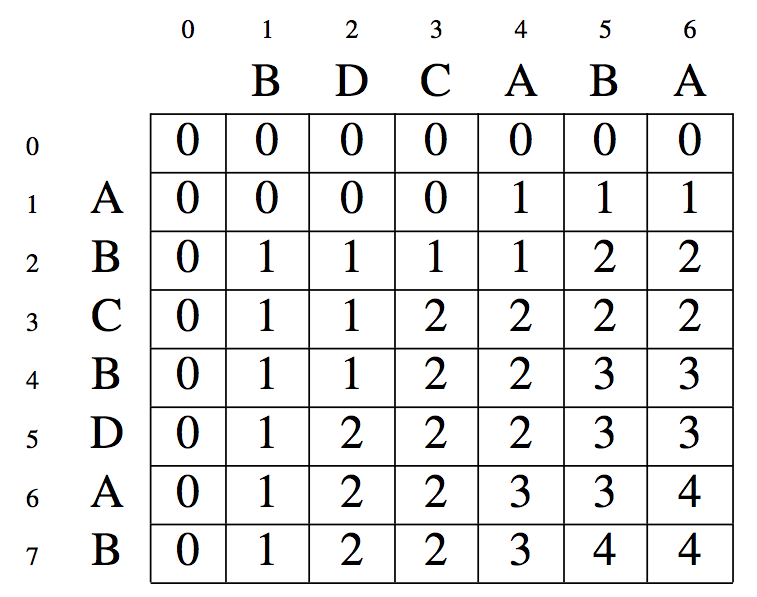
\includegraphics[width=0.35\textwidth]{img/matrix_1.png}
  \caption{Filled matrix after LCS algorithm.~\cite{esquema}.}
   \label{fig:1}
\end{figure}

With this matrix it is only needed that we start from the highest number and walk to the left. We go to the upper diagonal if there is a mismatch between the numbers and left only if they match.

\begin{figure}[h!]
  \centering
      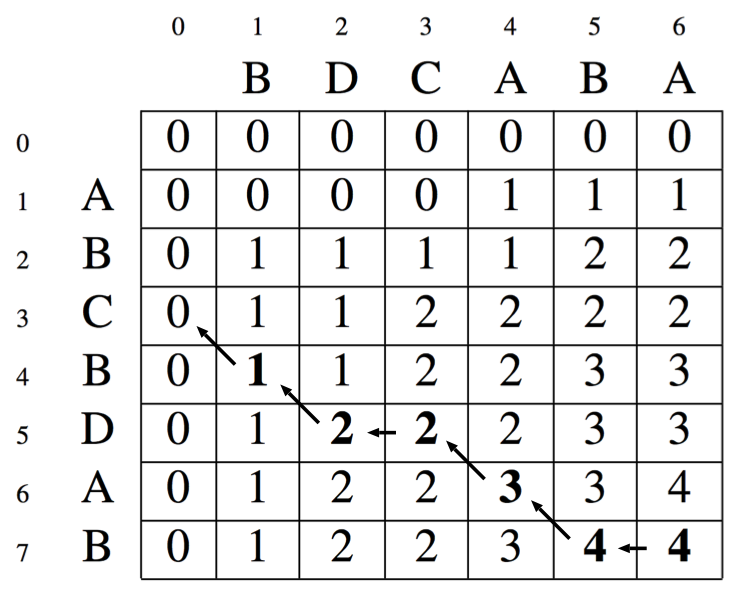
\includegraphics[width=0.35\textwidth]{img/matrix_2.png}
  \caption{Representation of the LCS walk.~\cite{esquema}.}
   \label{fig:2}
\end{figure}

We can achieve the LCS by selecting the letters corresponding to the indexes that make our walk move in the upper diagonal direction.
\section{Methods}
\subsection{Serial Implementation}
The implemented serial version was straightforward to implemente. The matrix was calculated element by element, line by line, taking advantage of the cache's Locality Principal, both spacial and temporal.
\vspace{2mm}

\begin{algorithm}
\caption{Serial LCS implementation}
\label{lcs-serial}
\begin{algorithmic}
\FOR{$i=0$ to $N$}
	\FOR{$j=0$ to $M$}
		\STATE Compute $C(i,j)$
	\ENDFOR
\ENDFOR
\end{algorithmic}
\end{algorithm}

Although this is the easiest solution to implement, it is not the best solution when it comes to transforming the code into an effective paralellized version.
%\begin{figure}[h!]
%  \centering
%      \includegraphics[width=0.5\textwidth]{esquema.png}
%  \caption{Circuito utilizado na constru��o da coluna~\cite{esquema}.}
%   \label{fig:2}
%\end{figure}

\subsection{Parallel Implementation}


\section{Results}
METER AQUI AS TABELAS COM OS VALORES

\section{Discussion}
DISCUTIR AQUI AS TABELAS

\section{Conclusions}
CONCLUIR CENAS

\vspace{-2mm}
\section{Agradecimentos}
We would like thank Professor Jos� Monteiro te


\begin{thebibliography}{99}

\bibitem{esquema}
K. Cantrell, "A Study of the Plasma Tweeter", B.Sc. Thesis, Ball State University (2011)

\bibitem{ideia}
M. Hopkins and T. Houlhan, "The Plasma Speaker: Construction and Characterization of both Full-bridge and Single-ended driving circuits", Project Report, University of Illinois at Urbana-Champaign (2012)

\bibitem{ideiageral}
D. Severinsen and G. Sen Gupta, "Design and Evaluation of Electronic Circuit for Plasma Speaker", Proceedings of the World Congress on Engineering 2013 Vol II (2013)

\bibitem{arstuff}
L. Wayne Sieck, John T. Herron, and David S. Green, Plasma Chem., Plasma P., Vol. 20, No. 2, 2000
\bibitem{arstuff2}
John T. Herron and David S. Green, Plasma Chem., Plasma P., Vol. 21, No. 3, 2001
\bibitem{arstuff3}
K.H. Becker, U. Kogelschatz, K.H. Schoenbach, R.J. Barker, "Non-Equilibrium Air Plasmas at Atmospheric Pressure", p. 130, Institute of Physics Publishing, Bristol, UK (2005)
\bibitem{Mathematica}
Wolfram Research, Inc., Mathematica, Version 9.0, Champaign, IL (2012).
\end{thebibliography}

\end{document}
